\documentclass{article}
\usepackage{tikz}
\usetikzlibrary{shapes.geometric, arrows}

\usepackage[a4paper, portrait, margin=1.5cm]{geometry}

% begin flow chart blocks
\tikzstyle{startstop} = [rectangle, rounded corners, 
minimum width=3cm, minimum height=1cm,
text centered, text width=3cm,
draw=black, fill=red!30]

\tikzstyle{io} = [trapezium, 
trapezium stretches=true,
trapezium left angle=70, 
trapezium right angle=110, 
minimum width=3cm, minimum height=1cm, 
text centered, text width=3cm, 
draw=black, fill=blue!30]

\tikzstyle{process} = [rectangle, 
minimum width=3cm, minimum height=1cm, 
text centered, text width=3cm, 
draw=black, fill=orange!30]

\tikzstyle{decision} = [diamond,
aspect = 2,
minimum width=3cm, minimum height=1cm, 
text centered, text width=2.5cm,
draw=black, fill=green!30]
\tikzstyle{arrow} = [thick,->,>=stealth]
% end flow chart blocks

\title{Preparing ('Digitizing') Images with Inkscape / Inkstitch for Machine Embroidery}
\author{Harald Kraft}
\date{\today}

\begin{document}

    \maketitle

    \tableofcontents

    \pagebreak

    \section{Prerequisites}
        \subsection{Inkscape}

        \subsection{Inkstitch}
    
        \pagebreak
    \section{Workflow}
        \subsection{Overview}
        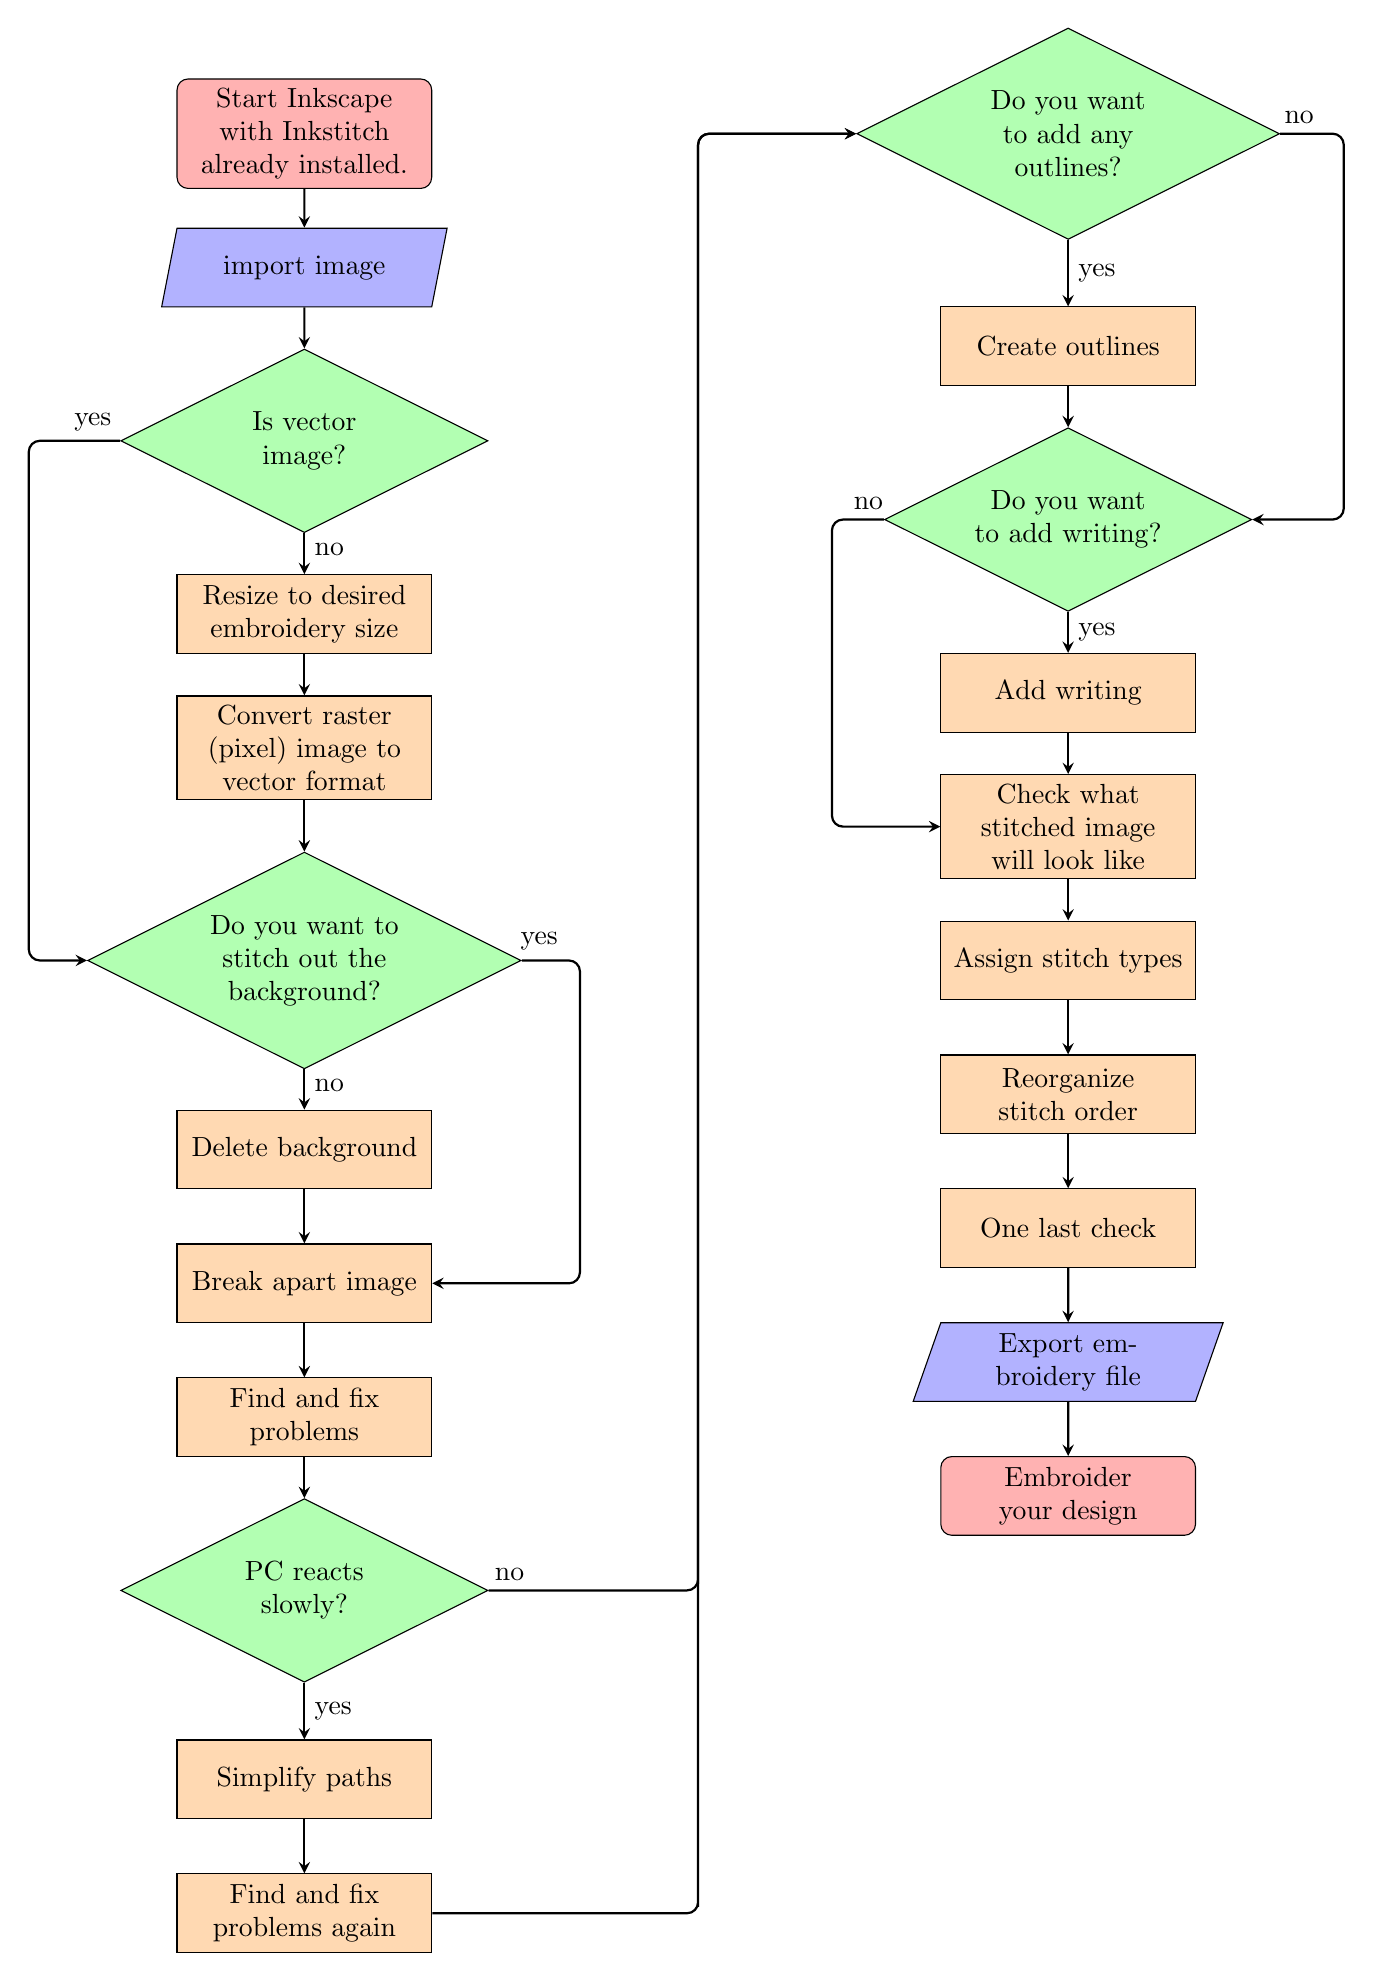
\begin{tikzpicture}[node distance=1.7cm]
            \node (start) [startstop] {Start Inkscape with Inkstitch already installed.};
            \node (import) [io, below of=start] {import image};
            \node (isVector) [decision, below of=import, yshift=-0.5cm] {Is vector image?};
            \node (resize) [process, below of=isVector, yshift=-0.5cm] {Resize to desired embroidery size};
            \node (conv) [process, below of=resize] {Convert raster (pixel) image to vector format};
            \node (backgr) [decision, below of=conv, yshift=-1cm] {Do you want to stitch out the background?};
            \node (delBackgr) [process, below of=backgr, yshift=-0.7cm] {Delete background};
            \node (split) [process, below of=delBackgr] {Break apart image};
            \node (trouble) [process, below of=split] {Find and fix problems};
            \node (slow) [decision, below of=trouble, yshift=-0.5cm] {PC reacts slowly?};
            \node (simplify) [process, below of=slow, yshift=-0.7cm] {Simplify paths};
            \node (troubleAgain) [process, below of=simplify] {Find and fix problems again};
            \node (wantOutlines) [decision, right of=start, xshift=8cm] {Do you want to add any outlines?};
            \node (outlines) [process, below of=wantOutlines, yshift=-1cm] {Create outlines};
            \node (wantLettering) [decision, below of=outlines, yshift=-0.5cm] {Do you want to add writing?};
            \node (lettering) [process, below of=wantLettering, yshift=-0.5cm] {Add writing};
            \node (check) [process, below of=lettering] {Check what stitched image will look like};
            \node (types) [process, below of=check] {Assign stitch types};
            \node (order) [process, below of=types] {Reorganize stitch order};
            \node (lastCheck) [process, below of=order] {One last check};
            \node (export) [io, below of=lastCheck] {Export embroidery file};
            \node (embroider) [startstop, below of=export] {Embroider your design};
            
            
            \draw [arrow] (start) -- (import);

            \draw [arrow] (import) -- (isVector);

            \draw [arrow] (isVector) -- node[pos=0.4, right] {no} (resize);
            \draw [arrow, rounded corners=4pt] (isVector) -- ++ (-3.5,0) node[pos=0.3, above] {yes} |- (backgr);

            \draw [arrow] (resize) -- (conv);

            \draw [arrow] (conv) -- (backgr);

            \draw [arrow] (backgr) -- node[pos=0.4, right] {no} (delBackgr);
            \draw [arrow, rounded corners=4pt] (backgr) -- ++ (3.5,0) node[pos=0.3, above] {yes} |- (split);

            \draw [arrow] (delBackgr) -- (split);
            
            \draw [arrow] (split) -- (trouble);

            \draw [arrow] (trouble) -- (slow);

            \draw [arrow] (slow) -- node[pos=0.5, right] {yes} (simplify);
            \draw [arrow, rounded corners=4pt](slow) -| ++ (5,0) node[pos=0.05, above] {no} |-(wantOutlines);
            
            \draw [arrow] (simplify) -- (troubleAgain);

            \draw [arrow, rounded corners=4pt] (troubleAgain) -| ++ (5,0) |- (wantOutlines);

            \draw [arrow] (wantOutlines) -- node[anchor=west] {yes} (outlines);
            \draw [arrow, rounded corners=4pt] (wantOutlines) -- ++ (3.5,0) node[pos=0.3, above] {no} |- (wantLettering);

            \draw [arrow] (outlines) -- (wantLettering);
            
            \draw [arrow] (wantLettering) -- node[anchor=west] {yes} (lettering);
            \draw [arrow, rounded corners=4pt] (wantLettering) -- ++ (-3,0) node[pos=0.3, above] {no} |- (check);

            \draw[arrow] (lettering) -- (check);

            \draw [arrow] (check) -- (types);

            \draw [arrow] (types) -- (order);

            \draw [arrow] (order) -- (lastCheck);

            \draw [arrow] (lastCheck) -- (export);

            \draw [arrow] (export) -- (embroider);

            \end{tikzpicture}

        \pagebreak

        \subsection{Import Image}
        
        \subsection{File Types}
            \subsubsection{Vector Formats}
            \subsubsection{Raster Formats}
        
        \subsection{Resizing}
        
        \subsection{Conversion to Vector Image}
        Trace Bitmap    

        \subsection{Delete Background}
        \subsubsection{Delete Background Layer}
        \subsubsection{Delete "Holes"}        
        
        \subsection{Break Apart Image}

        \subsection{Finding and fixing Problems}
            \subsubsection{Troubleshooter}
            \subsubsection{Clean up Document}
            \subsubsection{Small Infill}
            \subsubsection{Border Crosses Itself}
            \subsubsection{Rung Intersects Rail more than Once (Satin Stitch)}

        \subsection{Simplify Paths}
        
        \subsection{Finding and Fixing Problems, Again}

        \subsection{Creating Outlines}
        
        \subsection{Adding Writing / Lettering}

        \subsection{Checking what the Stitched Image will look like}
        
        \subsection{Assigning Stitch Types}
            \subsubsection{Straight Stitch}
            \subsubsection{Satin Stitch}
            \subsubsection{Fill Stitch}
        
        \subsection{Reorganizing the Stitch Order}
            \subsubsection{Grouping same Colour Parts}
            \subsubsection{Avoiding visible Jump Stitches}
        
        \subsection{One last Check}
        
        \subsection{Exporting to a File your Embroidery Machine can understand}
\end{document}